\section{Travail réalisé}

    \subsection{Organisation} 

        Notre objectif pour ce second semestre d’étude pratique était d’implémenter l’algorithme. Nous avons décidé de travailler chacun de notre côté dans un premier temps, car nous ne connaissions pas suffisamment le fonctionnement de Weka et le travail semblait difficilement sécable. Cette approche nous a effectivement permis de nous familiariser individuellement avec la bibliothèque Weka et nous avons chacun travaillé sur un début d’implémentation de VFDR.

        Nous nous sommes ensuite réunis pour comparer nos avancées respectives et nos choix d’implémentation. Nous avons décidé de conserver les choix faits par Clément, qui avait déjà bien avancé dans l’implémentation de l’algorithme. C’est donc la base que nous avons choisie pour terminer le travail du semestre.

    \begin{figure}
        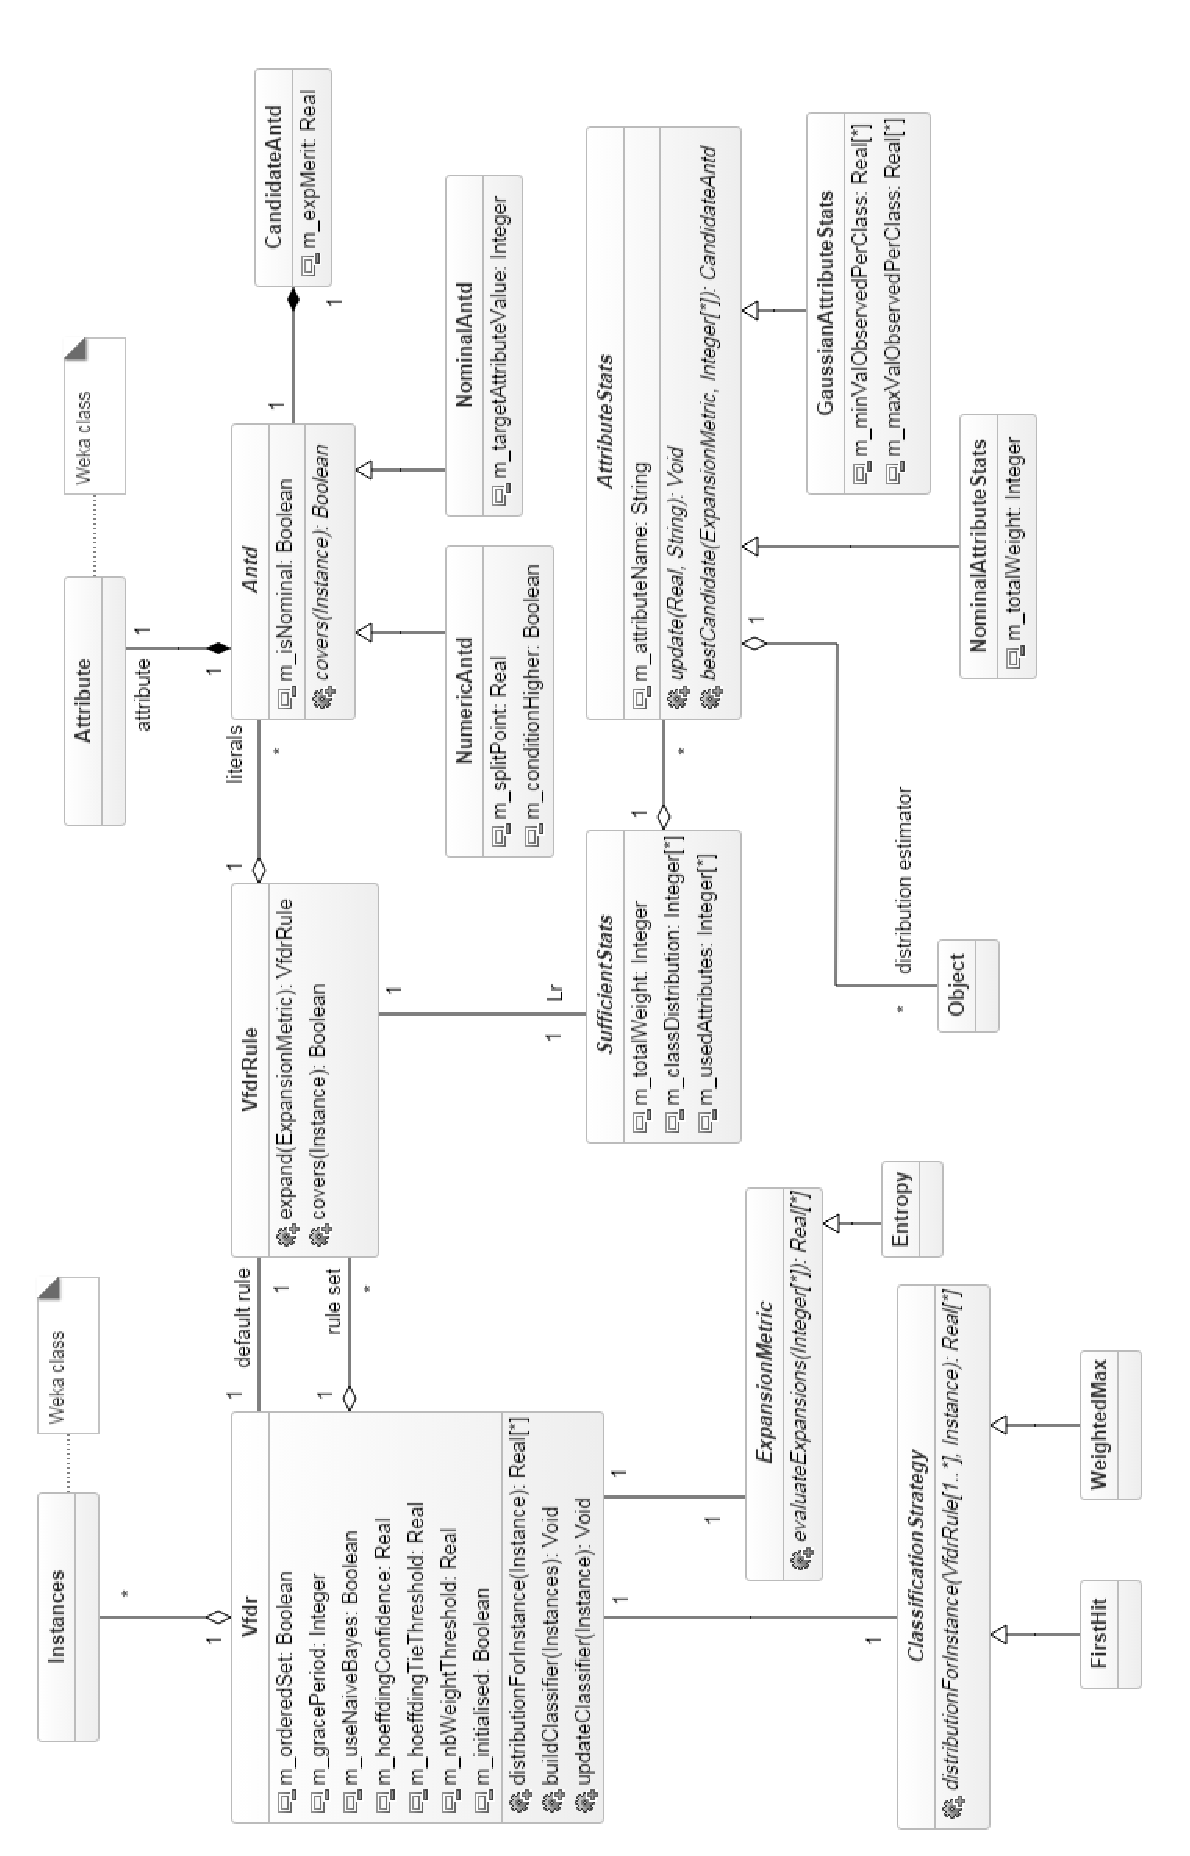
\includegraphics[width=\textwidth]{src/image2}
        \caption{Diagramme de classes de notre implémentation}
        \label{fig:dclass}
    \end{figure}


    \subsection{Description de l'implémentation}

        Le diagramme de classes en figure \ref{fig:dclass} présente l'architecture de notre implémentation.

        \paragraph{Paramétrage} La classe principale de notre programme, nommée \texttt{Vfdr}, implémente plusieurs interfaces de Weka, notamment UpdateableClassifier, qui permet de mettre en avant l’aspect incrémental de l’algorithme. Ces interfaces permettent d'intégrer le programme au GUI de Weka. \texttt{Vfdr} possède des attributs servant d’options de configuration, ainsi qu’une liste de \texttt{VfdrRule}, représentant l’ensemble des règles et une \texttt{VfdrRule} à part qui est la règle par défaut.

        \paragraph{Règles}Chaque objet \texttt{VfdrRule} possède lui-même une liste d’\texttt{Antd}, une classe abstraite servant à représenter les antécédents possibles pour les règles (spécialisée en \texttt{NumericAntd} pour les conditions sur les attributs numériques et \texttt{NominalAntd} pour les conditions sur les attributs nominaux). \texttt{VfdrRule} possède aussi une référence vers un objet \texttt{SufficientStats}, qui stocke les statistiques associées à la règle. 


        \paragraph{Statistiques suffisantes} 
            Dans l’implémentation, nous avons choisi d’identifier les classes des exemples par des Strings (le nom de la classe). Par conséquent, dans \texttt{SufficientStats}, le nombre d’exemples couverts par classe est stocké dans une \texttt{Map<String, Integer>}. Pour ce qui est des attributs, ils peuvent être représentés par des entiers (leur indice). On utilise par exemple une \texttt{List<Integer>} pour stocker les attributs déjà utilisés dans \texttt{SufficientStats}. Cependant, les attributs sont parfois identifiés par leur nom, comme les classes : les statistiques par attributs sont stockés dans une \texttt{Map<String, \texttt{AttributeStats}>}, où \texttt{AttributeStats} est une classe abstraite qui a des spécialisations différentes selon le type d’attribut.
            
            Pour gérer les statistiques des attributs numériques, certaines descriptions de l'algorithme VFDR indiquent d’utiliser un arbre binaire qui stocke pour chaque attribut la chance de rencontrer une valeur supérieure à chaque valeur déjà rencontrée. Pour simplifier l’implémentation, nous avons plutôt utilisé une densité de probabilité pour représenter les valeurs rencontrées : c’est la classe \texttt{GaussianAttributeStats}, qui hérite de \texttt{AttributeStats}. Les calculs sont faits dans la classe interne \texttt{GaussianEstimator}, qui hérite de la classe Weka \texttt{UnivariateNormalEstimator}. Ce choix a aussi l’avantage de limiter la complexité en temps et en espace.
        
        \paragraph{Expansion d'une règle} Pour l’expansion d’une règle, une liste de \texttt{CandidateAntd} (antécédents candidats) est créée. Le score de chaque candidat est évalué à l’aide d’un objet \texttt{ExpansionMetric}. Notons qu’\texttt{ExpansionMetric} est une classe abstraite, mais qu’elle n’a qu’une seule spécialisation possible : \texttt{Entropy}, qui utilise des calculs d’entropie pour évaluer la qualité d’une séparation. La mise en place d’une classe abstraite permet de laisser la possibilité d’améliorer l’implémentation, en ajoutant d'autres méthodes d’évaluation de séparation, tout en limitant les modifications à apporter au code existant.
        
        \paragraph{Prédiction} Lorsque l’on demande au \texttt{Vfdr} de classifier un exemple via la méthode \texttt{distributionForInstance}, sa stratégie de classification (représentée par la classe abstraite ClassificationStrategy) entre en jeu. Pour les ensembles ordonnés de règles, la stratégie est de type \texttt{FirstHit}, on renvoie la classe donnée par la première règle qui couvre l’exemple. Pour les ensembles non ordonnés, la stratégie est de type \texttt{WeightedMax}, on choisit alors la classe à partir de la règle qui couvre l’exemple et a le poids le plus élevé (le plus grand nombre total d’exemples couverts).

    \subsection{Limites de cette implémentation}

        Le temps de traitement d'un individu est suffisamment bas pour qu'il ne constitue pas un problème. Cependant la routine d'expansion de règle est très coûteuse et constitue le principal goulot d'étranglement pour le temps d'exécution du programme. Pour cette raison, nous avons défini une borne inférieure au nombre d'exemples que l'algorithme doit voir passer avant de tenter l'expansion. Cette limite est configurable et doit être adaptée au nombre d'exemples de l'échantillon d'apprentissage.

        Ll’algorithme ne peut pas gérer de changement de la fonction cible (ce que l'on appelle la \emph{dérive de concept}). Il existe une variante de l'algorithme qui peut s'y adapter, mais son implémentation était hors du champ de cette étude pratique.